\chapter{Diseño e implementación} % Main chapter title

\label{Chapter3} % Change X to a consecutive number; for referencing this chapter elsewhere, use \ref{ChapterX}

En este capítulo se presentan los detalles técnicos de diseño e implementación de la solución IoT que se tuvieron en cuenta durante el desarrollo del trabajo.


\section{Arquitectura de software del sistema}


El sistema cuenta con una arquitectura robusta y flexible en la que se integra el dispositivo robótico de exploración ambiental \citep{cese_gonzalo_memoria} desarrollado en el marco de la Carrera de Especialización en Sistemas Embebidos, con un sistema \textit{back-end} desplegado en la nube pública \citep{nube_publica}, y una red Blockchain \cite{blockchain} a fin de poder asegurar la inmutabilidad y transparencia de las lecturas ambientales. 


\section{Hardware e infraestructura del sistema}
 
 
\section{Integración de los módulos y subsistemas}




\subsection{Capa de percepción}


El desarrollo e integración de los componentes de esta capa consistió en la adaptación del firmware desplegado en el robot explorador para extender sus funcionalidades y enviar las lecturas de parámetros ambientales al \textit{topic} MQTT. Dentro de las funcionalidades que se le agregaron al robot explorador se encontraron:

\begin{itemize}
	\item Capturar fecha y hora local del sistema.
	\item Generación de coordenadas geograficas (con datos \textit{mock}).
	\item Conexión segura con tópico MQTT y envío de los datos generados.	
		
\end{itemize}

La configuración de la fecha y hora se realizó por medio del uso del servicio SNTP \citep{sntp} que permite la sincronización del hardware de una red con la fecha y hora provista por servicios externos en estandar en una zona horaria. Esta configuración se realizó incluyendo el encabezado \textbf{esp\_sntp.h} en el código del robot. Una vez realizado esto fue posible obtener la fecha y hora local invocando a la función \textit{localtime}.

La generación de las coordenadas geograficas con datos \textit{mock} se realizo mediante la generación de las ecuaciones \ref{eq:mock_lat} y \ref{eq:mock_long} a continuación.

\begin{equation}
	\label{eq:mock_lat}
	MockLat = \left( \frac{rand()}{RAND\_MAX} \right) \left( LAT\_MAX - LAT\_MIN \right) + LAT\_MIN
\end{equation}
                
\begin{equation}
	\label{eq:mock_long}
	MockLong = \left( \frac{rand()}{RAND\_MAX} \right) \left( LONG\_MAX - LONG\_MIN \right) + LONG\_MIN
\end{equation}

Finalmente, los datos capturados fueron enviados en formato JSON al tópico MQTT con la estructura de la tabla:


\begin{table}[h]
	\centering
	\caption[caption corto]{Tabla de objetos AWS}
	\begin{tabular}{l c c}    
		\toprule
		\textbf{Nombre del campo} & \textbf{Tipo del campo} & \textbf{Descripción}  \\
		\midrule
		deviceId & string & Id del dispositivo \\		
		type & string & Tipo de lectura \\		
		value & string & Valor de la lectura \\		
		geoLat & string & Latitud geográfica \\		
		geoLong & string & Longitud geográfica\\		
		date & string & Fecha \\		
		time & string & Hora \\		
		
		\bottomrule
		\hline
	\end{tabular}
	\label{tab:json_fields}
\end{table}


A continuación podemos apreciar un valor de ejemplo del objeto JSON enviado por el robot:

\begin{lstlisting}
{   	
	"deviceId": "12ad-dao23-ux23",
	"type": "Temperature",
	"value": "0.00",
	"geoLat": "-26.056772",
	"geoLong": "-64.014824",
	"date": "2025-04-1",
	"time": "11:23:59"
}
\end{lstlisting}

\subsection{Capa de red}

El desarrollo de los componentes de esta capa consistió en la publicación de un \textit{topic} MQTT desde el servicio AWS IoT Core y la configuración de la lógica de redirección y almacenamiento de los mensajes recibidos en AWS S3.


Para la conexión segura con el tópico MQTT se configuró el servicio AWS IoT Core, donde se creó una nueva instancia de un dispositivo remoto con el nombre ESP32. Una vez creado este dispositivo se descargaron e instalaron en el código del robot los certificados listados a continuación:




\begin{itemize}
	\item AmazonRootCA1.pem, renombrado a brokerCA.crt:	Es la autoridad certificadora que AWS usa para firmar certificados de sus servidores. El dispositivo lo necesita para verificar la identidad del servidor AWS IoT al conectarse.
	\item dev-certificate.pem.crt, renombrado a client.crt: Contiene la clave pública correspondiente a la clave privada (.key) y está firmado por AWS (o por una CA en la que AWS confía) para verificar la identidad del dispositivo.
	\item dev-private.pem.key, renombrado a client.key: Usada por el dispositivo para firmar su identidad durante la conexión TLS. Nunca se comparte ni se sube a AWS. Tu dispositivo la usa para autenticar su certificado (.crt).
		
\end{itemize}

Una vez realizada la configuración del servicio AWS IoT core e integrado el robot con el tópico, se probó la recepción de lecturas con el cliente de prueba provisto por AWS suscrito al tópico \textit{readings} como puede apreciarse en la figura \ref{fig:aws_iot_core_mqtt_test_2}.

\begin{center}
   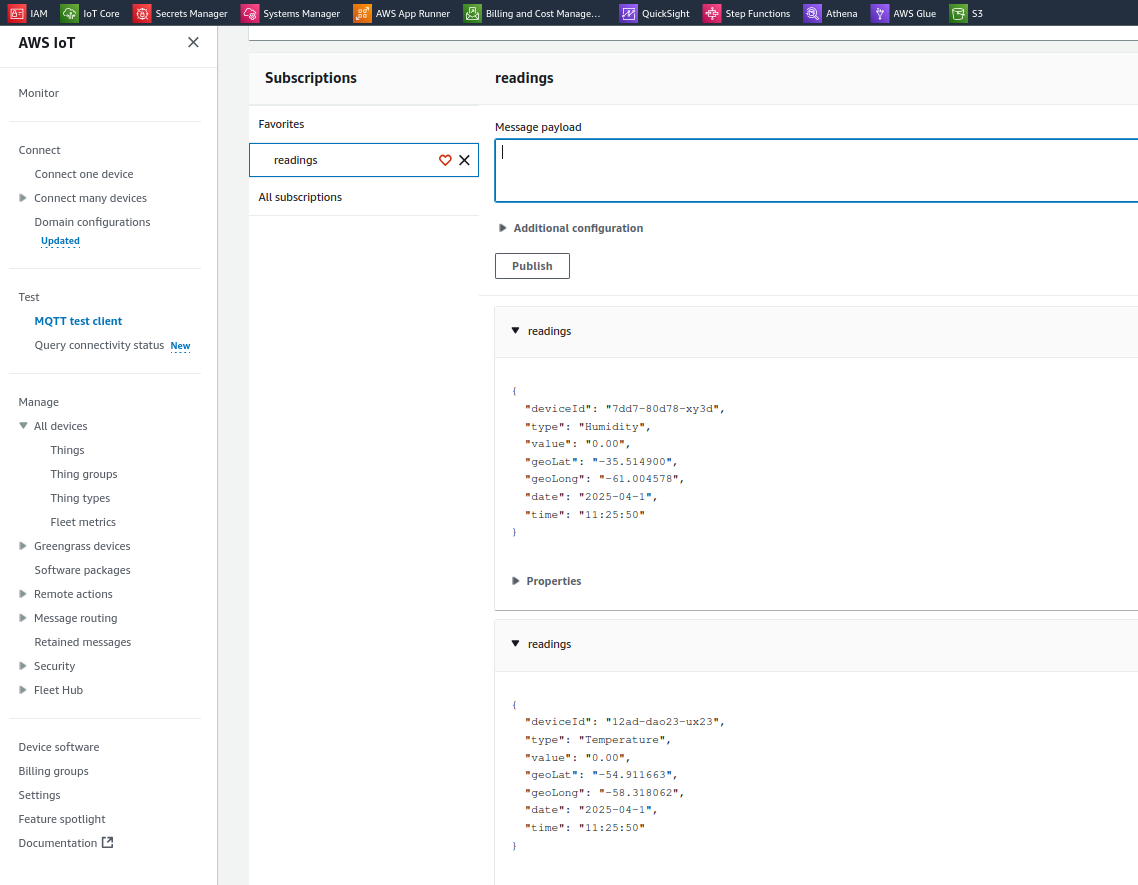
\includegraphics[scale=0.35]{AWS/aws_iot_core_mqtt_test_2}
   \captionof{figure}{Prueba de recepción de mensajes MQTT.}
   \label{fig:aws_iot_core_mqtt_test_2}
\end{center}

Para el almacenamiento en AWS S3 de los mensajes recibidos, se configuro una \textit{routing rule} o regla de redirección en AWS IoT Core, indicando mediante una consulta con sintaxis SQL, que todos los mensajes recibidos en el tópico \textit{readings} deben almacernarce en el bucket S3 ceiot-exploratory-robot. En la figura \ref{fig:aws_iot_core_message_routing} puede apreciarse esta configuración.
 

\begin{center}
   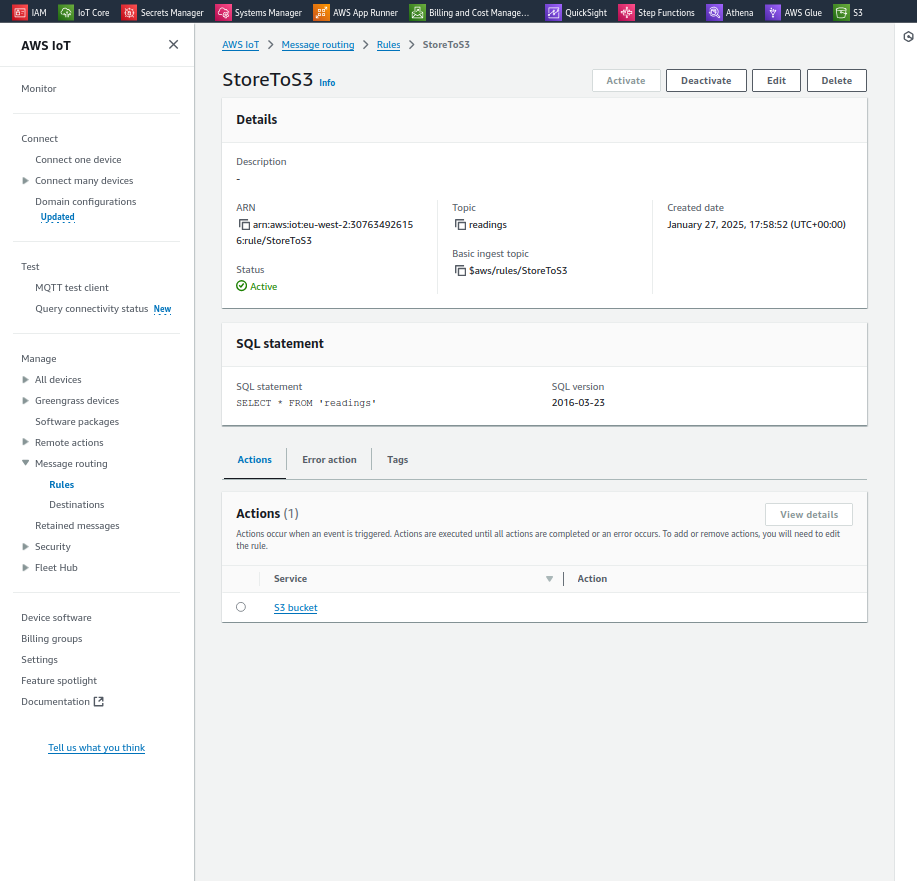
\includegraphics[scale=0.4]{AWS/aws_iot_core_message_routing}
   \captionof{figure}{Configuración de redirección de mensajes MQTT.}
   \label{fig:aws_iot_core_message_routing}
\end{center}

Como resultado de la configuración realizada, los mensajes recibidos en MQTT fueron redirigidos y almacenados en AWS S3 como puede apreciarse en la figura \ref{fig:aws_s3_bucket_data2}.

\begin{center}
   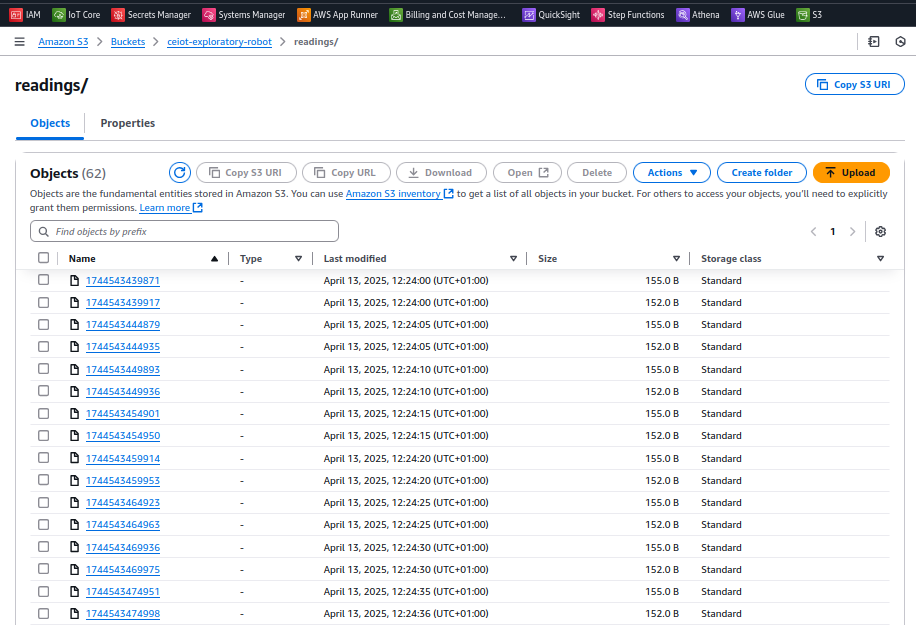
\includegraphics[scale=0.4]{AWS/aws_s3_bucket_data2}
   \captionof{figure}{Almacenamiento de mensajes JSON en AWS S3.}
   \label{fig:aws_s3_bucket_data2}
\end{center}


\subsection{Capas de procesamiento y almacenamiento - cloud}

Una vez realizadas las configuraciones de ingesta de datos en \textit{streaming} se realizaron las configuraciones para poder administrarlos y procesarlos.
Para ello se crearon una base de datos y una tabla en AWS Glue para representar el esquema de datos almacenados en AWS S3 en formato JSON, como se puede apreciar en la figura \ref{fig:aws_glue_table_review}.

\begin{center}
   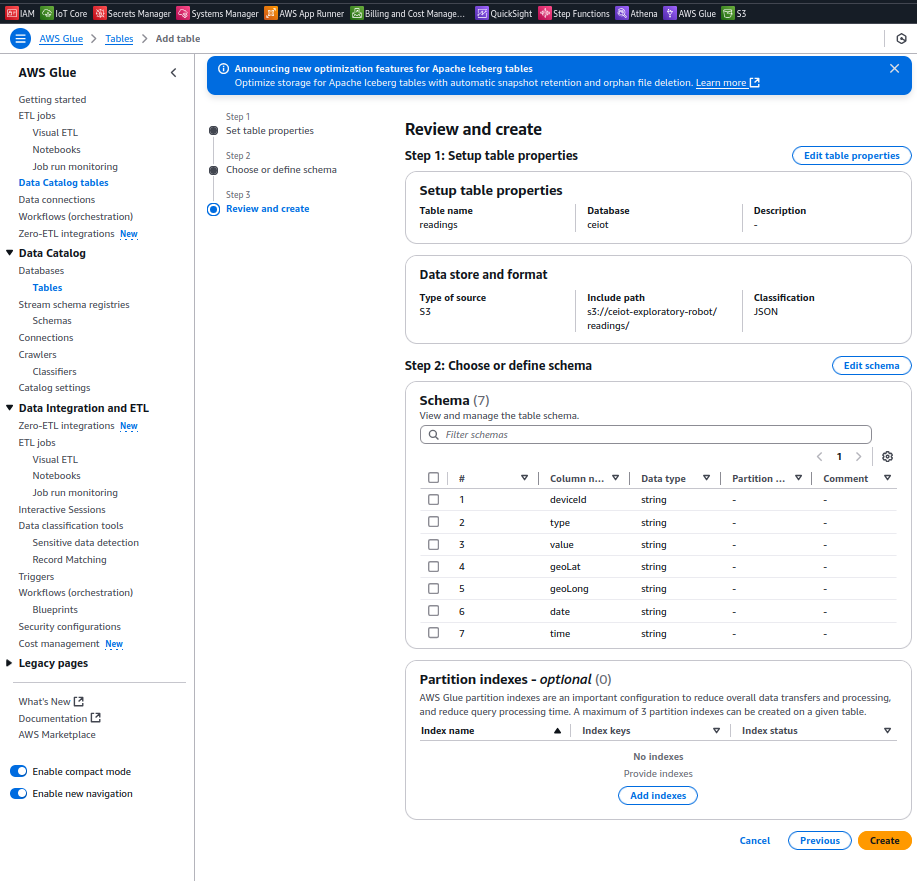
\includegraphics[scale=0.4]{AWS/aws_glue_table_review}
   \captionof{figure}{Creación de base datos, tabla y esquema AWS Glue.}
   \label{fig:aws_glue_table_review}
\end{center}

Con el esquema de datos definido en el catálogo de AWS Glue, fue posible realizar consultas SQL sobre los datos almacenados en AWS S3 desde AWS Athena, como se puede apreciar en la figura 

\begin{center}
   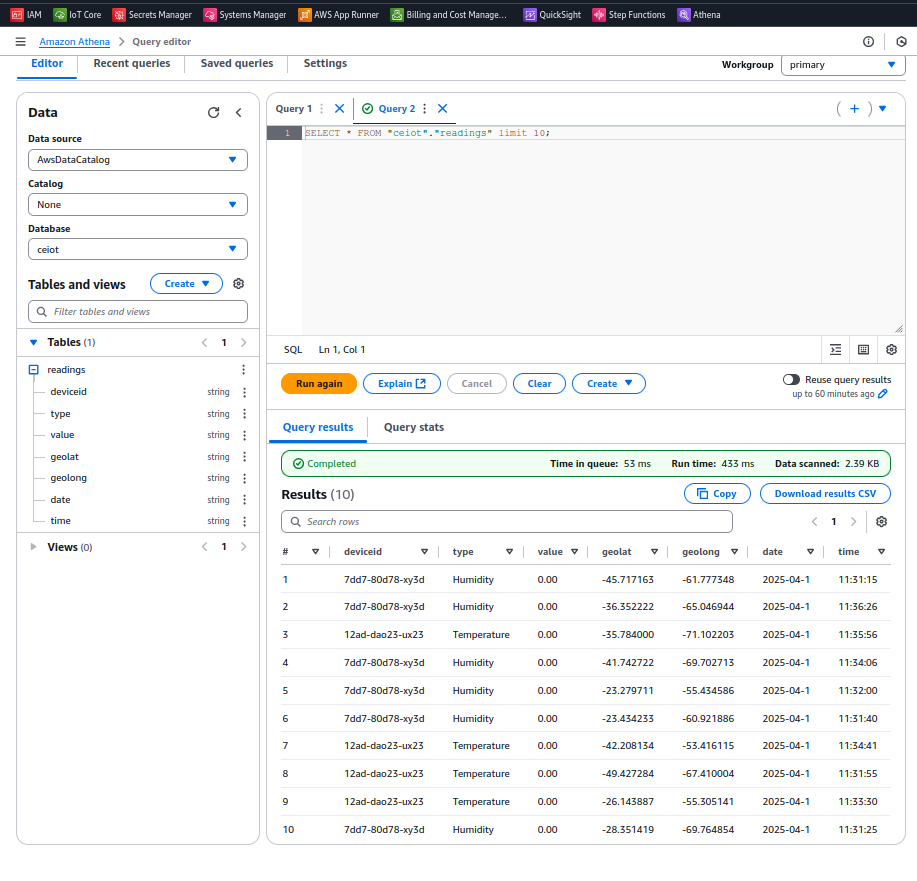
\includegraphics[scale=0.4]{AWS/aws_athena_config}
   \captionof{figure}{Consulta de datos SQL desde AWS Athena.}
   \label{fig:aws_athena_config}
\end{center}





\subsection{Capas de procesamiento y almacenamiento - blockchain}

La capa de procesamiento y almacenamiento blockchain esta formada por los componentes \textit{smart contracts} y la dApp que los accede.

Para el desarrollo de los \textit{smart contracts} se utilizó Solidity como lenguaje de programanción y Truffle como herramienta de gestión de configuración, compilación, empaquetado y despliegue. Truffle utiliza una configuración basada en archivos Javascript para la descripción de las tareas, y para realizar el despliegue a diferentes redes, como por ejemplo de forma local a Ganache o de forma remota a redes como Sepolia, Holesky y Mainnet.

El proceso de desarrollo de 


Desde el punto de vista del \textit{backend} blockchain, se desarrollo la dApp utilizando Node.js y la biblioteca Javascript Web3.js para la comunicación con los \textit{smart contracts}.

Se desarrollaron varios \textit{endpoints} listados a continuacion en la siguiente tabla:

'
'
'
'

Para el acceso a los \textit{smart contracts} la dApp necesita tener disponible los archivos ABI generados en la compilacion.



\section{Plataforma de desarrollo y despliegue}



\section{Tabla de todos los objetos AWS creados}




\begin{table}[h]
	\centering
	\caption[caption corto]{Tabla de objetos AWS}
	\begin{tabular}{l c c}    
		\toprule
		\textbf{Servicio} & \textbf{Propósito} & \textbf{Nombre de objeto}  \\
		\midrule
		AWS IoT Core & \textit{Thing} & ESP32 \\		
		AWS IoT Core & \textit{MQTT topic} & /readings \\		
		AWS IoT Core & \textit{Routing Rule} & StoreToS3 \\		
		AWS S3 & Bucket & ceiot-exploratory-robot \\		
		\bottomrule
		\hline
	\end{tabular}
	\label{tab:peces}
\end{table}

